\section{Exercises}

%__________________
\subsection{Normal distribution}

% 1

\eoce{\qt{Area under the curve, I} What percent of a standard normal distribution $N(\mu=0, \sigma=1)$ is found in each region? Be sure to draw a graph. \vspace{-3mm}
\begin{multicols}{4}
\begin{parts}
\item $Z < -1.35$
\item $Z > 1.48$
\item $-0.4 < Z < 1.5$
\item $|Z| > 2$
\end{parts}
\end{multicols}
}{}

% 2

\eoce{\qt{Area under the curve, II} What percent of a standard normal distribution $N(\mu=0, \sigma=1)$ is found in each region? Be sure to draw a graph. \vspace{-3mm}
\begin{multicols}{4}
\begin{parts}
\item $Z > -1.13$
\item $Z < 0.18$
\item $Z > 8$
\item $|Z| < 0.5$
\end{parts}
\end{multicols}
}{}

% 3

\eoce{\qt{Scores on the GRE, Part I\label{GRE}} A college senior who took the Graduate Record Examination exam scored 620 on the Verbal Reasoning section and 670 on the Quantitative Reasoning section. The mean score for Verbal Reasoning section was 462 with a standard deviation of 119, and the mean score for the Quantitative Reasoning was 584 with a standard deviation of 151. Suppose that both distributions are nearly normal.
\begin{parts}
\item Write down the short-hand for these two normal distributions.
\item What is her Z score on the Verbal Reasoning section? On the Quantitative Reasoning section? Draw a standard normal distribution curve and mark these two Z scores.
\item What do these Z scores tell you?
\item Relative to others, which section did she do better on?
\item Find her percentile scores for the two exams.
\item What percent of the test takers did better than her on the Verbal Reasoning section? On the Quantitative Reasoning section?
\item Explain why simply comparing her raw scores from the two sections would lead to the incorrect conclusion that she did better on the Quantitative Reasoning section.
\item If the distributions of the scores on these exams are not nearly normal, would your answers to parts (b) - (f) change? Explain your reasoning.
\end{parts}
}{}

% 4

\eoce{\qt{Triathlon times, Part I} \label{triathlon} In triathlons, it is common for racers to be placed into age and gender groups. Friends Leo and Mary both completed the Hermosa Beach Triathlon, where Leo competed in the \textit{Men, Ages 30 - 34} group while Mary competed in the \textit{Women, Ages 25 - 29} group. Leo completed the race in 1:22:28 (4948 seconds), while Mary completed the race in 1:31:53 (5513 seconds). Obviously Leo finished faster, but they are curious about how they did within their respective groups. Can you help them?
Here is some information on the performance of their groups:
\begin{itemize}
\setlength{\itemsep}{0mm}
\item The finishing times of the \textit{Men, Ages 30 - 34} group has a mean of 4313 seconds with a standard deviation of 583 seconds.
\item The finishing times of the \textit{Women, Ages 25 - 29} group has a mean of 5261 seconds with a standard deviation of 807 seconds.
\item The distributions of finishing times for both groups are approximately Normal.
\end{itemize}
Remember: a better performance corresponds to a faster finish.
\begin{parts}
\item Write down the short-hand for these two normal distributions.
\item What are the Z scores for Leo's and Mary's finishing times? What do these Z scores tell you?
\item Did Leo or Mary rank better in their respective groups? Explain your reasoning.
\item What percent of the triathletes did Leo finish faster than in his group?
\item What percent of the triathletes did Mary finish faster than in her group?
\item If the distributions of finishing times are not nearly normal, would your answers to parts (b) - (e) change? Explain your reasoning.
\end{parts}
}{}

% 5

\eoce{\qt{GRE scores, Part II} In Exercise~\ref{GRE} we saw two distributions for GRE scores: $N(\mu=462, \sigma=119)$ for the verbal part of the exam and $N(\mu=584, \sigma=151)$ for the quantitative part. Use this information to compute each of the following:
\begin{parts}
\item The score of a student who scored in the $80^{th}$ percentile on the Quantitative Reasoning section.
\item The score of a student who scored worse than 70\% of the test takers in the Verbal Reasoning section.
\end{parts}
}{}

% 6

\eoce{\qt{Triathlon times, Part II} In Exercise~\ref{triathlon} we saw two distributions for triathlon times: $N(\mu=4313, \sigma=583)$ for \emph{Men, Ages 30 - 34} and $N(\mu=5261, \sigma=807)$ for the \emph{Women, Ages 25 - 29} group. Times are listed in seconds. Use this information to compute each of the following:
\begin{parts}
\item The cutoff time for the fastest 5\% of athletes in the men's group, i.e. those who took the shortest 5\% of time to finish. 
\item The cutoff time for the slowest 10\% of athletes in the women's group. 
\end{parts}
}{}

% 7

\eoce{\qt{Temperatures in LA, Part I} \label{tempLA} The average daily high temperature in June in LA is 77\degree F with a standard deviation of 5\degree F. Suppose that the temperatures in June closely follow a normal distribution. 
\begin{parts}
\item What is the probability of observing an 83\degree F temperature or higher in LA during a randomly chosen day in June?
\item How cold are the coldest 10\% of the days during June in LA?
\end{parts}
}{}

% 8

\eoce{\qt{Portfolio returns} The Capital Asset Pricing Model is a financial model that assumes returns on a portfolio are normally distributed. Suppose a portfolio has an average annual return of 14.7\% (i.e. an average gain of 14.7\%) with a standard deviation of 33\%. A return of 0\% means the value of the portfolio doesn't change, a negative return means that the portfolio loses money, and a positive return means that the portfolio gains money.
\begin{parts}
\item What percent of years does this portfolio lose money, i.e. have a return less than 0\%?
\item What is the cutoff for the highest 15\% of annual returns with this portfolio?
\end{parts}
}{}

% 9

\eoce{\qt{Temperatures in LA, Part II} Exercise~\ref{tempLA} states that average daily high temperature in June in LA is 77\degree F with a standard deviation of 5\degree F, and it can be assumed that they to follow a normal distribution. We use the following equation to convert \degree F (Fahrenheit) to \degree C (Celsius):
\[ C = (F - 32) \times \frac{5}{9}. \]
\begin{parts}
\item Write the probability model for the distribution of temperature in \degree C in June in LA.
\item What is the probability of observing a 28\degree C (which roughly corresponds to 83\degree F) temperature or higher in June in LA? Calculate using the \degree C model from part (a).
\item Did you get the same answer or different answers in part (b) of this question and part (a) of Exercise~\ref{tempLA}? Are you surprised? Explain.
\end{parts}
}{}

% 10

\eoce{\qt{Heights of 10 year olds} Heights of 10 year olds, regardless of gender, closely follow a normal distribution with mean 55 inches and standard deviation 6 inches.
\begin{parts}
\item What is the probability that a randomly chosen 10 year old is shorter than 48 inches?
\item What is the probability that a randomly chosen 10 year old is between 60 and 65 inches?
\item If the tallest 10\% of the class is considered ``very tall", what is the height cutoff for ``very tall"?
\item The height requirement for \textit{Batman the Ride} at Six Flags Magic Mountain is 54 inches. What percent of 10 year olds cannot go on this ride?
\end{parts}
}{}

% 11

\eoce{\qt{Auto insurance premiums} Suppose a newspaper article states that the distribution of auto insurance premiums for residents of California is approximately normal with a mean of \$1,650. The article also states that 25\% of California residents pay more than \$1,800. 
\begin{parts}
\item What is the Z score that corresponds to the top 25\% (or the $75^{th}$ percentile) of the standard normal distribution?
\item What is the mean insurance cost? What is the cutoff for the 75th percentile?
\item Identify the standard deviation of insurance premiums in LA.
\end{parts}
}{}

% 12

\eoce{\qt{Speeding on the I-5, Part I} \label{i5} The distribution of passenger vehicle speeds traveling on the Interstate 5 Freeway (I-5) in California is nearly normal with a mean of 72.6 miles/hour and a standard deviation of 4.78 miles/hour.\footfullcite{Johnson+Murray:2010}
\begin{parts}
\item What percent of passenger vehicles travel slower than 80 miles/hour?
\item What percent of passenger vehicles travel between 60 and 80 miles/hour?
\item How fast do the fastest 5\% of passenger vehicles travel?
\item The speed limit on this stretch of the I-5 is 70 miles/hour. Approximate what percentage of the passenger vehicles travel above the speed limit on this stretch of the I-5.
\end{parts}
}{}

% 13

\eoce{\qt{Overweight baggage} Suppose weights of the checked baggage of airline passengers follow a nearly normal distribution with mean 45 pounds and standard deviation 3.2 pounds. Most airlines charge a fee for baggage that weigh in excess of 50 pounds. Determine what percent of airline passengers incur this fee.
}{}

% 14

\eoce{\qt{Find the SD} Find the standard deviation of the distribution in the following situations.
\begin{parts}
\item  MENSA is an organization whose members have IQs in the top 2\% of the population. IQs are normally distributed with mean 100, and the minimum IQ score required for admission to MENSA is 132.
\item Cholesterol levels for women aged 20 to 34 follow an approximately normal distribution with mean 185 milligrams per deciliter (mg/dl). Women with cholesterol levels above 220 mg/dl are considered to have high cholesterol and about 18.5\% of women fall into this category.
\end{parts}
}{}

% 15

\eoce{\qt{Buying books on Ebay} The textbook you need to buy for your chemistry class is expensive at the college bookstore, so you consider buying it on Ebay instead. A look at past auctions suggest that the prices of that chemistry textbook have an approximately normal distribution with mean \$89 and standard deviation \$15. 
\begin{parts}

\item What is the probability that a randomly selected auction for this book closes at more than \$100?

\item Ebay allows you to set your maximum bid price so that if someone outbids you on an auction you can automatically outbid them, up to the maximum bid price you set. If you are only bidding on one auction, what are the advantages and disadvantages of setting a bid price too high or too low? What if you are bidding on multiple auctions?

\item If you watched 10 auctions, roughly what percentile might you use for a maximum bid cutoff to be somewhat sure that you will win one of these ten auctions? Is it possible to find a cutoff point that will ensure that you win an auction?

\item If you are willing to track up to ten auctions closely, about what price might you use as your maximum bid price if you want to be somewhat sure that you will buy one of these ten books?

\end{parts}
}{}

% 16

\textB{\pagebreak}

\eoce{\qt{SAT scores} SAT scores (out of 2400) are distributed normally with a mean of 1500 and a standard deviation of 300. Suppose a school council awards a certificate of excellence to all students who score at least 1900 on the SAT, and suppose we pick one of the recognized students at random. What is the probability this student's score will be at least 2100? (The material covered in Section~\ref{conditionalProbabilitySection} would be useful for this question.)
}{}

% 17

\eoce{\qt{Scores on stats final, Part I} \label{statsScores} Below are final exam scores of 20 Introductory Statistics students. 
\[ \stackrel{1}{57}, \stackrel{2}{66}, \stackrel{3}{69}, \stackrel{4}{71}, \stackrel{5}{72}, \stackrel{6}{73}, \stackrel{7}{74}, \stackrel{8}{77}, \stackrel{9}{78}, \stackrel{10}{78}, \stackrel{11}{79}, \stackrel{12}{79}, \stackrel{13}{81}, \stackrel{14}{81}, \stackrel{15}{82}, \stackrel{16}{83}, \stackrel{17}{83}, \stackrel{18}{88}, \stackrel{19}{89}, \stackrel{20}{94} \]
The mean score is 77.7 points. with a standard deviation of 8.44 points. Use this information to determine if the scores approximately follow the 68-95-99.7\% Rule.
}{}

% 18

\eoce{\qt{Heights of female college students, Part I} \label{collegeFemHeights} Below are heights of 25 female college students.
\[ \stackrel{1}{54}, \stackrel{2}{55}, \stackrel{3}{56}, \stackrel{4}{56}, \stackrel{5}{57}, \stackrel{6}{58}, \stackrel{7}{58}, \stackrel{8}{59}, \stackrel{9}{60}, \stackrel{10}{60}, \stackrel{11}{60}, \stackrel{12}{61}, \stackrel{13}{61}, \stackrel{14}{62}, \stackrel{15}{62}, \stackrel{16}{63}, \stackrel{17}{63}, \stackrel{18}{63}, \stackrel{19}{64}, \stackrel{20}{65}, \stackrel{21}{65}, \stackrel{22}{67}, \stackrel{23}{67}, \stackrel{24}{69}, \stackrel{25}{73} \]
The mean height is 61.52 inches with a standard deviation of 4.58 inches. Use this information to determine if the heights approximately follow the 68-95-99.7\% Rule.
}{}


%__________________
\subsection{Evaluating the Normal approximation}

% 19

\eoce{\qt{Scores on stats final, Part II} Exercise~\ref{statsScores} lists the final exam scores of 20 Introductory Statistics students. Do these data appear to follow a normal distribution? Explain your reasoning using the graphs provided below.
\begin{center}
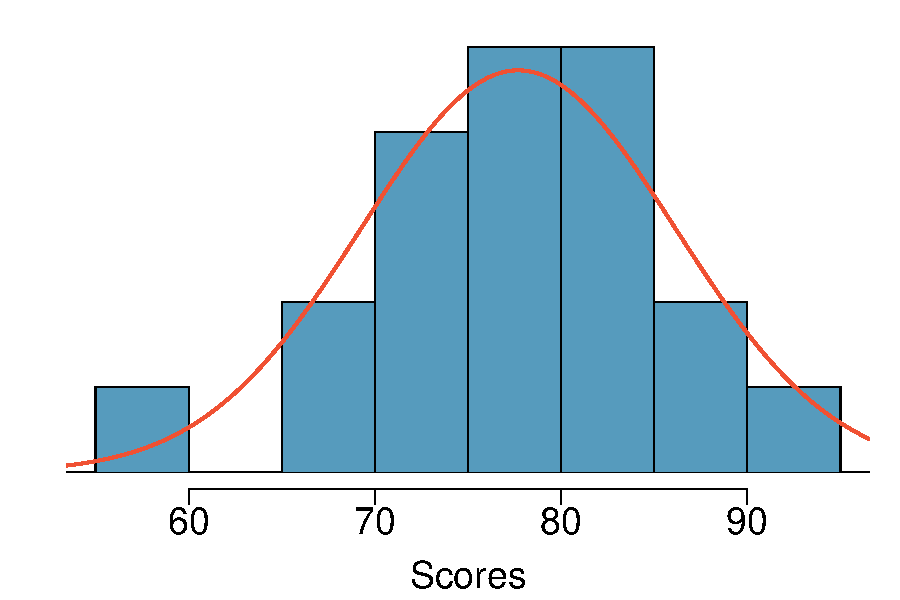
\includegraphics[width=0.46\textwidth]{03/figures/eoce/scores/scores_hist}\ \ \ \ 
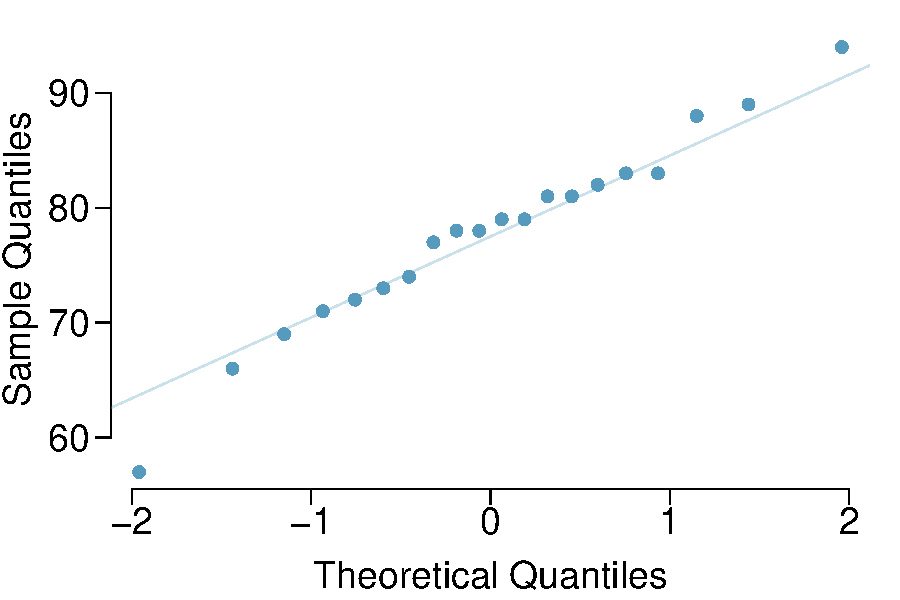
\includegraphics[width= 0.46\textwidth]{03/figures/eoce/scores/scores_qq}
\end{center}
}{}

% 20

\eoce{\qt{Heights of female college students, Part II} Exercise~\ref{collegeFemHeights} lists the heights of 25 female college students. Do these data appear to follow a normal distribution? Explain your reasoning using the graphs provided below.
\begin{center}
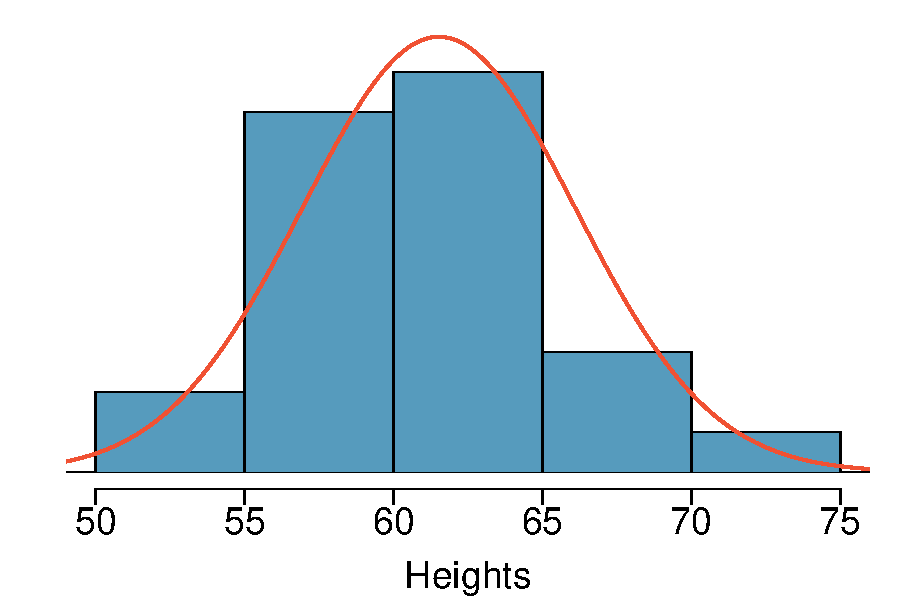
\includegraphics[width= 0.46\textwidth]{03/figures/eoce/heightsFcoll/heightsFcoll_hist}\ \ \ \ 
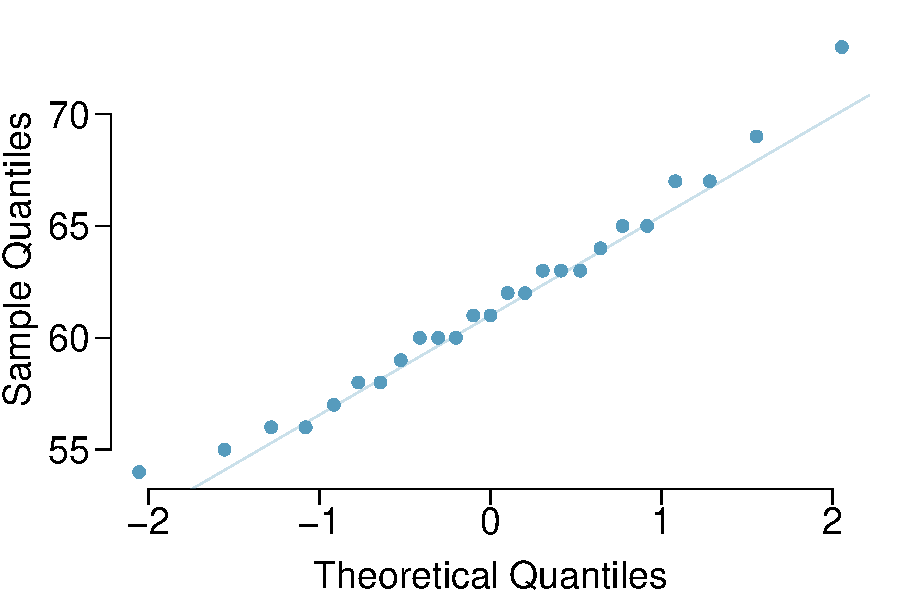
\includegraphics[width= 0.46\textwidth]{03/figures/eoce/heightsFcoll/heightsFcoll_qq}
\end{center}
}{}

\textB{\pagebreak}


%__________________
\subsection{Geometric distribution}

% 21

\eoce{\qtq{Is it Bernoulli} Determine if each trial can be considered an independent Bernouilli trial for the following situations.
\begin{parts}
\item Cards dealt in a hand of poker.
\item Outcome of each roll of a die.
\end{parts}
}{}

% 22

\eoce{\qt{With and without replacement} In the following situations assume that half of the specified population is male and the other half is female.
\begin{parts}
\item Suppose you're sampling from a room with 10 people. What is the probability of sampling two females in a row when sampling with replacement? What is the probability when sampling without replacement?
\item Now suppose you're sampling from a stadium with 10,000 people. What is the probability of sampling two females in a row when sampling with replacement? What is the probability when sampling without replacement?
\item We often treat individuals who are sampled from a large population as independent. Using your findings from parts~(a) and~(b), explain whether or not this assumption is reasonable.
\end{parts}
}{}

% 23

\eoce{\qt{Married women} \label{marriedWomen} The 2010 American Community Survey estimates that 47.1\% of women ages 15 years and over are married.\footfullcite{marWomenACS}
\begin{parts}
\item We randomly select three women between these ages. What is the probability that the third woman selected is the only one who is married?
\item What is the probability that all three randomly selected women are married?
\item On average, how many women would you expect to sample before selecting a married woman? What is the standard deviation?
\item If the proportion of married women was actually 30\%, how many women would you expect to sample before selecting a married woman? What is the standard deviation?
\item Based on your answers to parts (c) and (d), how does decreasing the probability of an event affect the mean and standard deviation of the wait time until success?
\end{parts}
}{}

% 24

\eoce{\qt{Defective rate} \label{transistorLow} A machine that produces a special type of transistor (a component of computers) has a 2\% defective rate. The production is considered a random process where each transistor is independent of the others.
\begin{parts}
\item What is the probability that the $10^{th}$ transistor produced is the first with a defect?
\item What is the probability that the machine produces no defective transistors in a batch of 100?
\item On average, how many transistors would you expect to be produced before the first with a defect? What is the standard deviation?
\item Another machine that also produces transistors has a 5\% defective rate where each transistor is produced independent of the others. On average how many transistors would you expect to be produced with this machine before the first with a defect? What is the standard deviation?
\item Based on your answers to parts (c) and (d), how does increasing the probability of an event affect the mean and standard deviation of the wait time until success?
\end{parts}
}{}

\textB{\pagebreak}

% 25

\eoce{\qt{Eye color, Part I} \label{eyeColor} A husband and wife both have brown eyes but carry genes that make it possible for their children to have brown eyes (probability 0.75), blue eyes (0.125), or green eyes (0.125). \vspaceB{-0.5mm}
\begin{parts}
\item What is the probability the first blue-eyed child they have is their third child? Assume that the eye colors of the children are independent of each other.
\item On average, how many children would such a pair of parents have before having a blue-eyed child? What is the standard deviation of the number of children they would expect to have until the first blue-eyed child?
\end{parts}
}{}

% 26

\eoce{\qt{Speeding on the I-5, Part II} \label{i5Geom} Exercise~\ref{i5} states that the distribution of speeds of cars traveling on the Interstate 5 Freeway (I-5) in California is nearly normal with a mean of 72.6 miles/hour and a standard deviation of 4.78 miles/hour. The speed limit on this stretch of the I-5 is 70 miles/hour. \vspaceB{-0.5mm}
\begin{parts}
\item A highway patrol officer is hidden on the side of the freeway. What is the probability that 5~cars pass and none are speeding? Assume that the speeds of the cars are independent of each other.
\item On average, how many cars would the highway patrol officer expect to watch until the first car that is speeding? What is the standard deviation of the number of cars he would expect to watch?
\end{parts}
}{}


%__________________
\subsection{Binomial distribution}

% 27

\eoce{\qt{Underage drinking, Part I} \label{alcohol} The Substance Abuse and Mental Health Services Administration estimated that 70\% of 18-20 year olds consumed alcoholic beverages in 2008.\footfullcite{webpage:alcohol} \vspaceB{-0.5mm}
\begin{parts}
\item Suppose a random sample of ten 18-20 year olds is taken. Is the use of the binomial distribution appropriate for calculating the probability that exactly six consumed alcoholic beverages? Explain.
\item Calculate the probability that exactly 6 out of 10 randomly sampled 18-20 year olds consumed an alcoholic drink.
\item What is the probability that exactly four out of the ten 18-20 year olds have \textit{not} consumed an alcoholic beverage?
\item What is the probability that at most 2 out of 5 randomly sampled 18-20 year olds have consumed alcoholic beverages?
\item What is the probability that at least 1 out of 5 randomly sampled 18-20 year olds have consumed alcoholic beverages?
\end{parts}
}{}

% 28

\eoce{\qt{Chickenpox, Part I} \label{chickenpox} The National Vaccine Information Center estimates that 90\% of Americans have had chickenpox by the time they reach adulthood.  \footfullcite{webpage:chickenpox} \vspaceB{-0.5mm}
\begin{parts}
\item Suppose we take a random sample of 100 American adults. Is the use of the binomial distribution appropriate for calculating the probability that exactly 97 had chickenpox before they reached adulthood? Explain.
\item Calculate the probability that exactly 97 out of 100 randomly sampled American adults had chickenpox during childhood.
\item What is the probability that exactly 3 out of a new sample of 100 American adults have \textit{not} had chickenpox in their childhood?
\item What is the probability that at least 1 out of 10 randomly sampled American adults have had chickenpox?
\item What is the probability that at most 3 out of 10 randomly sampled American adults have \textit{not} had chickenpox?
\end{parts}
}{}

% 29

\eoce{\qt{Underage drinking, Part II} We learned in Exercise~\ref{alcohol} that about 70\% of 18-20 year olds consumed alcoholic beverages in 2008. We now consider a random sample of fifty 18-20 year olds.
\begin{parts}
\item How many people would you expect to have consumed alcoholic beverages? And with what standard deviation?
\item Would you be surprised if there were 45 or more people who have consumed alcoholic beverages?
\item What is the probability that 45 or more people in this sample have consumed alcoholic beverages? How does this probability relate to your answer to part (b)?
\end{parts}
}{}

% 30

\eoce{\qt{Chickenpox, Part II} We learned in Exercise~\ref{chickenpox} that about 90\% of American adults had chickenpox before adulthood. We now consider a random sample of 120 American adults.
\begin{parts}
\item How many people in this sample would you expect to have had chickenpox in their childhood? And with what standard deviation?
\item Would you be surprised if there were 105 people who have had chickenpox in their childhood?
\item What is the probability that 105 or fewer people in this sample have had chickenpox in their childhood? How does this probability relate to your answer to part (b)?
\end{parts}
}{}

% 31
\eoce{\qt{University admissions} Suppose a university announced that it admitted 2,500 students for the following year's freshman class. However, the university has dorm room spots for only 1,786 freshman students. If there is a 70\% chance that an admitted student will decide to accept the offer and attend this university, what is the approximate probability that the university will not have enough dormitory room spots for the freshman class?
}{}


% 32

\eoce{\qt{Survey response rate} Pew Research reported in 2012 that the typical response rate to their surveys is only 9\%. If for a particular survey 15,000 households are contacted, what is the probability that at least 1,500 will agree to respond? \footfullcite{surveysPew}
}{}

% 33

\eoce{\qt{Game of dreidel} A dreidel is a four-sided spinning top with the Hebrew letters \textit{nun}, \textit{gimel}, \textit{hei}, and \textit{shin}, one on each side. Each side is equally likely to come up in a single spin of the dreidel. Suppose you spin a dreidel three times. Calculate the probability of getting\footfullcite{dreidelPic}

\noindent\begin{minipage}[c]{0.75\textwidth}
%\begin{multicols}{2}
\begin{parts}
\item at least one \textit{nun}? 
\item exactly 2 \textit{nun}s? 
\item exactly 1 \textit{hei}? 
\item at most 2 \textit{gimel}s? 
\end{parts} \vspace{6mm}
%\end{multicols}
\end{minipage}%
\begin{minipage}[c]{0.25\textwidth} \ \\[2mm]
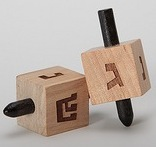
\includegraphics[width=0.85\textwidth]{03/figures/eoce/images/dreidelSm}
\end{minipage}
}{}

% 34

\eoce{\qt{Arachnophobia} A 2005 Gallup Poll found that that 7\% of teenagers (ages 13 to 17) suffer from arachnophobia and are extremely afraid of spiders. At a summer camp there are 10 teenagers sleeping in each tent. Assume that these 10 teenagers are independent of each other.\footfullcite{webpage:spiders}
\begin{parts}
\item Calculate the probability that at least one of them suffers from arachnophobia.
\item Calculate the probability that exactly 2 of them suffer from arachnophobia?
\item Calculate the probability that at most 1 of them suffers from arachnophobia? 
\item If the camp counselor wants to make sure no more than 1 teenager in each tent is afraid of spiders, does it seem reasonable for him to randomly assign teenagers to tents?
\end{parts}
}{}

% 35

\eoce{\qt{Eye color, Part II} Exercise~\ref{eyeColor} introduces a husband and wife with brown eyes who have 0.75 probability of having children with brown eyes, 0.125 probability of having children with blue eyes, and 0.125 probability of having children with green eyes.
\begin{parts}
\item What is the probability that their first child will have green eyes and the second will not?
\item What is the probability that exactly one of their two children will have green eyes?
\item If they have six children, what is the probability that exactly two will have green eyes?
\item If they have six children, what is the probability that at least one will have green eyes?
\item What is the probability that the first green eyed child will be the $4^{th}$ child? 
\item Would it be considered unusual if only 2 out of their 6 children had brown eyes?
\end{parts}
}{}

% 36

\eoce{\qt{Sickle cell anemia} Sickle cell anemia is a genetic blood disorder where red blood cells lose their flexibility and assume an abnormal, rigid, ``sickle" shape, which results in a risk of various complications. If both parents are carriers of the disease, then a child has a 25\% chance of having the disease, 50\% chance of being a carrier, and 25\% chance of neither having the disease nor being a carrier. If two parents who are carriers of the disease have 3 children, what is the probability that 
\begin{parts}
\item two will have the disease?
\item none will have the disease?
\item at least one will neither have the disease nor be a carrier?
\item the first child with the disease will the be $3^{rd}$ child?
\end{parts}
}{}

% 37

\eoce{\qt{Roulette winnings} In the game of roulette, a wheel is spun and you place bets on where it will stop. One popular bet is that it will stop on a red slot; such a bet has an 18/38 chance of winning. If it stops on red, you double the money you bet. If not, you lose the money you bet. Suppose you play 3 times, each time with a \$1 bet. Let Y represent the total amount won or lost. Write a probability model for Y.
}{}

% 38

\eoce{\qt{Multiple choice quiz} In a multiple choice quiz there are 5 questions and 4 choices for each question (a, b, c, d). Robin has not studied for the quiz at all, and decides to randomly guess the answers. What is the probability that
\begin{parts}
\item the first question she gets right is the $3^{rd}$ question?
\item she gets exactly 3 or exactly 4 questions right?
\item she gets the majority of the questions right?
\end{parts}
}{}

% 39

\eoce{\qt{Exploring combinations} The formula for the number of ways to arrange $n$ objects is $n! = n\times(n-1)\times \cdots \times 2 \times 1$. This exercise walks you through the derivation of this formula for a couple of special cases.

\indent A small company has five employees: Anna, Ben, Carl, Damian, and Eddy. There are five parking spots in a row at the company, none of which are assigned, and each day the employees pull into a random parking spot. That is, all possible orderings of the cars in the row of spots are equally likely.
\begin{parts}
\item On a given day, what is the probability that the employees park in alphabetical order?
\item If the alphabetical order has an equal chance of occurring relative to all other possible orderings, how many ways must there be to arrange the five cars?
\item Now consider a sample of 8 employees instead. How many possible ways are there to order these 8 employees' cars?
\end{parts}
}{}

\textB{\pagebreak}

% 40

\eoce{\qt{Male children} While it is often assumed that the probabilities of having a boy or a girl are the same, the actual probability of having a boy is slightly higher at 0.51. Suppose a couple plans to have 3 kids. 
\begin{parts}
\item Use the binomial model to calculate the probability that two of them will be boys.
\item Write out all possible orderings of 3 children, 2 of whom are boys. Use these scenarios to calculate the same probability from part (a) but using the Addition Rule for disjoint events. Confirm that your answers from parts (a) and (b) match.
\item If we wanted to calculate the probability that a couple who plans to have 8 kids will have 3 boys, briefly describe why the approach from part (b) would be more tedious than the approach from part (a).
\end{parts}
}{}


%__________________
\subsection{More discrete distributions}

% 41

\eoce{\qt{Identify the distribution} Calculate the following probabilities and indicate which probability distribution model is appropriate in each case. You roll a fair die 5 times. What is the probability of rolling
\begin{parts}
\item the first 6 on the fifth roll?
\item exactly three 6s?
\item the third 6 on the fifth roll?
\end{parts}
}{}

% 42

\eoce{\qt{Darts} Calculate the following probabilities and indicate which probability distribution model is appropriate in each case. A very good darts player can hit the bullseye (red circle in the center of the dart board) 65\% of the time. What is the probability that he
\begin{parts}
\item hits the bullseye for the $10^{th}$ time on the $15^{th}$ try?
\item hits the bullseye 10 times in 15 tries?
\item hits the first bullseye on the third try?
\end{parts}
}{}

% 43

\eoce{\qt{Sampling at school} For a sociology class project you are asked to conduct a survey on 20 students at your school. You decide to stand outside of your dorm's cafeteria and conduct the survey on a random sample of 20 students leaving the cafeteria after dinner one evening. Your dorm is comprised of 45\% males and 55\% females.
\begin{parts}
\item Which probability model is most appropriate for calculating the probability that the $4^{th}$ person you survey is the $2^{nd}$ female? Explain.
\item Compute the probability from part (a).
\item The three possible scenarios that lead to $4^{th}$ person you survey being the $2^{nd}$ female are
\[ \{M, M, F, F\}, \{M, F, M, F\}, \{F, M, M, F\} \]
One common feature among these scenarios is that the last trial is always female. In the first three trials there are 2 males and 1 female. Use the binomial coefficient to confirm that there are 3 ways of ordering 2 males and 1 female. 
\item Use the findings presented in part (c) to explain why the formula for the coefficient for the negative binomial is ${n-1 \choose k-1}$ while the formula for the binomial coefficient is ${n \choose k}$.
\end{parts}
}{}

% 44

\eoce{\qt{Serving in volleyball} A not-so-skilled volleyball player has a 15\% chance of making the serve, which involves hitting the ball so it passes over the net on a trajectory such that it will land in the opposing team's court. Suppose that her serves are independent of each other.
\begin{parts}
\item What is the probability that on the $10^{th}$ try she will make her $3^{rd}$ successful serve?
\item Suppose she has made two successful serves in nine attempts. What is the probability that her $10^{th}$ serve will be successful?
\item Even though parts (a) and (b) discuss the same scenario, the probabilities you calculated should be different. Can you explain the reason for this discrepancy?
\end{parts}
}{}

% 45

\eoce{\qt{Customers at a coffee shop, Part I} \label{coffee} A coffee shop serves an average of 75 customers per hour during the morning rush.
\begin{parts}
\item Which distribution we have studied is most appropriate for calculating the probability of a given number of customers arriving within one hour during this time of day?
\item What are the mean and the standard deviation of the number of customers this coffee shop serves in one hour during this time of day?
\item Would it be considered unusually low if only 60 customers showed up to this coffee shop in one hour during this time of day?
\end{parts}
}{}

% 46

\eoce{\qt{Stenographer's typos, Part I} \label{steno} A very skilled court stenographer makes one typographical error (typo) per hour on average.
\begin{parts}
\item What probability distribution is most appropriate for calculating the probability of a given number of typos this stenographer makes in an hour?
\item What are the mean and the standard deviation of the number of typos this stenographer makes?
\item Would it be considered unusual if this stenographer made 4 typos in a given hour? 
\end{parts}
}{}


% 47

\eoce{\qt{Customers at a coffee shop, Part II} Exercise~\ref{coffee} gives the average number of customers visiting a particular coffee shop during the morning rush hour as 75. Calculate the probability that this coffee shop serves 70 customers in one hour during this time of day?
}{}


% 48

\eoce{\qt{Stenographer's typos, Part II} Exercise~\ref{steno} gives the average number of typos of a very skilled court stenographer as 1 per hour. Calculate the probability that this stenographer makes at most 2 typos in a given hour.
}{}
